\documentclass{article}
\usepackage{graphicx}
\usepackage{setspace}
\usepackage[most]{tcolorbox}
\usepackage[utf8]{inputenc}
\usepackage{titlesec}
\usepackage{geometry}
\usepackage{fancyhdr}
\usepackage{fancyvrb}
\usepackage{geometry} %setlength{skipfootins}{1cm} begin{document}
\pagestyle{fancy}
\usepackage{ragged2e}
\usepackage{tocloft}
\renewcommand{\contentsname}{\Huge \underline{CONTENTS}}
\titleformat{\section}[block]{\color{black}\LARGE\bfseries\filcenter}{}{1em}{}
\titleformat{\subsection}[hang]{\bfseries}{}{1em}{\underline}
\renewcommand{\cftsecfont}{\normalfont\large} 
\setcounter{secnumdepth}{0}
\newtcolorbox{mytextbox}[1][]{
  colframe=gray,
  enhanced,
  colback=white,
  height=5cm,
  attach title to upper
}
\begin{document}



\setlength{\headsep}{0.1in}

\centering
 {\Large DIVISION OF COMPUTER ENGINEERING\\ SCHOOL OF ENGINEERING\\ COCHIN UNIVERSITY OF SCIENCE\\ AND TECHNOLOGY\\ KOCHI-682022\\ }
 \begin{figure}[h]
     \centering
     \vspace{1cm}
     
\includegraphics[height=5cm]{logo.png}
 \end{figure}


{\large \vspace{1cm} \textbf{19-202-0408 DATABASE MANAGEMENT SYSTEMS LABORATORY} \singlespacing \textbf{LABORATORY RECORD \vspace{1cm}}
}

\begin{mytextbox}
\doublespacing
\textbf{\\ \textit{NAME:}} ABHIMANUE TD\singlespacing
\textbf{\textit{COURSE:}} B-TECH COMPUTER SCIENCE AND ENGINEERING\singlespacing
\textbf{\textit{SEMESTER:}} IV\singlespacing
\textbf{\textit{REGISTER NUMBER:}} 20222113
\end{mytextbox}
\pagestyle{empty}



\newpage
\begin{verbatim}
    
\end{verbatim}


\newpage
 {\Large DIVISION OF COMPUTER ENGINEERING\\ SCHOOL OF ENGINEERING\\ COCHIN UNIVERSITY OF SCIENCE\\ AND TECHNOLOGY\\ KOCHI-682022\\ }
 \begin{figure}[h]
     \centering
     \vspace{1cm}
     
\includegraphics[height=5cm]{logo.png}
 \end{figure}


{\large \vspace{1cm} \textbf{19-202-0408 DATABASE MANAGEMENT SYSTEMS LABORATORY} \singlespacing \textbf{LABORATORY RECORD \vspace{1cm}}
}
{\\ \large Certified that the this is the Bonafide Record of the experiments done by ABHIMANUE TD Register No.20222113 of IV Semester B-Tech Computer Science and Engineering during the year 2023-2024.}
\\
\vspace{3cm} \textbf{ \small{Faculty in charge\hspace{1cm}Internal Evaluator\hspace{1cm}End semester evaluator}}
\newpage
\fancyhead{}
\setcounter{tocdepth}{1}

\newpage
\begin{verbatim}
    
\end{verbatim}


\newpage
{\begin{flushleft}
\begin{center}
    \textbf{\Huge\underline {CONTENTS}}
\end{center}
\vspace{0.3in}\hspace{2.5in} \textbf{\Large CYCLE I}\\
\vspace{0.5in}1.\hspace{1in}INSTALLATION AND CONFIGURATION OF MySQL\\\hspace{1in} SERVER AND CLIENT.
NORMAL INSTALLATION,SECURE\\ \hspace{1in} INSTALLATION, EDITING CON-
FIGURATION FILE.\\ \vspace{-0.4in}\hspace{5.8in}9\\
\vspace{0.5in}2.\hspace{1in}CREATING DATABASES, DIFFERENT TYPES OF USERS\\\hspace{1in} AND SETTING UP PRIVILEGES.\\  \vspace{-0.3in}\hspace{5.8in}13\\
\vspace{0.5in}3.\hspace{1in}CREATING TABLES, INSERTING AND UPDATING VALUES.\hspace{0.7in}15\\
\vspace{0.5in}4.\hspace{1in}INSERTING AND UPDATING VALUES FROM OTHER\\ \hspace{1in} TABLES AND .csv FILES.\hspace{3.1in}21\\
\vspace{0.5in}5.\hspace{1in}SELECT QUERIES.\hspace{3.43in}25\\
\vspace{0.5in}6.\hspace{1in}JOIN TABLES.\hspace{3.74in}27\\
\vspace{0.5in}7.\hspace{1in}NORMALIZING TABLES.\hspace{3.04in}29\\
\vspace{0.5in}8.\hspace{1in}DUMP, IMPORT AND SOURCE IN MYSQL.\hspace{1.85in}31\\

\end{flushleft}}
\newpage
\textbf{ }
\newpage
{\begin{flushleft}
\begin{center}
    \textbf{\Huge\underline {CONTENTS}}
\end{center}
\vspace{0.3in}\hspace{2.5in} \textbf{\Large CYCLE II}\\
\vspace{0.5in}1.\hspace{1in}INSTALLING NGINX AND PHP. \hspace{2.5in}33\\
\vspace{0.5in}2.\hspace{1in}CONFIGURING NGINX AND PHP. \hspace{2.4in}35\\
\vspace{0.5in}3.\hspace{1in}CREATE A WEBPAGE FOR STUDENTS REGISTRATION\\\hspace{1in} WITH ALL THE FIELDS LR REQUIRED AS PER THE \\\hspace{1in}EXPERIMENT IN CYCLE NUMBER 1 FOR STUDENT DATA\\\hspace{1in} AND ALSO INCLUDE USERNAME AND
PASSWORD IN\\\hspace{1in} REGISTRATION FORM AND ALSO HASH THE PASSWORD\\ \vspace{-0.7in} \hspace{5.8in}39\\
\vspace{1in}4.\hspace{1in}CREATE A LOGIN PAGE THAT ACCEPTS THE USERNAME\\ \hspace{1in} AND PASSWORD FOR STUDENT DATA.IF SUCCESSFULL\\ \hspace{1in} LOGIN AND SHOW DETAILS.\\\vspace{-0.5in} \hspace{5.8in}43\\


\end{flushleft}}
\newpage
\textbf{ }
\newpage
  
\pagestyle{fancy}
\newpage
\fancyhead[LO]{\textbf{CYCLE-1, EXPERIMENT-1}}
\fancyhead[RO]{02/04/2024}


 \addcontentsline{toc}{section}{\Huge \\ Cycle-1 \vspace{0.5cm}}
\section{INSTALLATION AND CONFIGURATION OF MySQL SERVER AND CLIENT. NORMAL INSTALLATION, SECURE INSTALLATION, EDITING CONFIGURATION FILE}
\hrulefill
\vspace{1cm}
\begin{flushleft}

\subsection{AIM}

To install mysql server and client.\\i) Normal installation, ii) Secure installation, iii) Edit configuration files.

\subsection{PROCEDURE}
\textbf{{\normalsize i) NORMAL INSTALLATION}}\\
\vspace{0.1in}
\textbullet{ Installation of MySQL client and servers from Ubuntu's packages.\\}
\hspace{0.6in} \$sudo apt install mysql-server \\
\hspace{0.8in} \$sudo apt install mysql-client \\
\vspace{5pt}
\textbullet{ After completion then start the server service. \\}
\hspace{0.6in} \$sudo systemctl restart mysql\\
\textbullet{ In terminal access MySQL as the root\\}
\hspace{0.6in} \$sudo mysql \\ \vspace{5pt}
\textbullet{ Now set a new password to the root account \\}
\hspace{0.6in} \textgreater ALTER USER 'root@localhost' IDENTIFIED BY 'password';\\ \vspace{5pt}

\vspace{0.25in}
\textbf{{\normalsize ii) SECURE INSTALLATION}}\\
\vspace{0.1in}
\textbullet{ To secure installation: \\}
\hspace{0.6in} \$sudo mysql\_secure\_installation \\
\vspace{5pt}
\textbullet{ Option for change password of root \\}
\hspace{0.6in} \$Change the password for root ?\\ \vspace{0.1in}\hspace{0.7in}Press y/Y for Yes, any other key for No) : Y\\
\vspace{0.1in}\hspace{0.55in}\$New password: 
\hspace{0.6in}\$Re-enter new password:\\




\end{flushleft}
\newpage
\textbf{ }
\newpage
\begin{flushleft}
\textbullet{ Remove anonymous users \\ }
\hspace{0.6in}\$Remove anonymous users?\\ \vspace{0.1in}\hspace{0.7in}Press y for Yes, any other key for No) : N

\textbullet{ Disallow root login \\ }
\hspace{0.6in}\$Disallow root login remotely?\\ \vspace{0.1in}\hspace{0.7in}Press y for Yes, any other key for No) : N

\textbullet{ Remove test database \\} 
\hspace{0.6in}\$Remove test database and access to it?\\ \vspace{0.1in}\hspace{0.7in}Press y for Yes, any other key for No) : N

\textbullet{ Remove test database \\ }
\hspace{0.6in}\$Reload privilege tables now?\\ \vspace{0.1in}\hspace{0.7in}Press y for Yes, any other key for No) : Y\\ \vspace{0.1in}

\textbf{{\normalsize iii) EDIT CONFIGURATION FILES}}
\\ \vspace{0.1in}
\textbullet{ Directory /etc/mysql\\ }
\hspace{0.6in} \$sudo cd /etc/mysql/\\ 
\textbullet{ Configuration of file mysql.cnf in vim\\} 
\hspace{0.6in} \$vim mysql.cnf\\

\subsection{RESULT}
Installation of MySQL server and client with normal installation, secure installation and edit configuration files has been successful executed.


\end{flushleft}
\newpage
\fancyhead[LO]{\textbf{CYCLE-1, EXPERIMENT-2}}
\begin{verbatim}
Databases in MySQL 

>show databases
+--------------------+
| Database           |
+--------------------+
| information_schema |
| mysql              |
| performance_schema |
| sys                |
| abhimanue_20222113 |
+--------------------+

\end{verbatim}
\newpage
\begin{flushleft}
\section{CREATING DATABASES, DIFFERENT TYPES OF USERS AND SETTING UP PRIVILEGES}
\hrulefill
\vspace{1cm}

\subsection{AIM}
To create different types of users,create a database and grant required privileges for the user on the database.
\subsection{PROCEDURE}
\subsubsection{Types of user}
\vspace{0.1in}\texttt{Global user}\\
\hspace{0.5in} \$sudo mysql -u root -p'password'\\
\hspace{0.6in} \textgreater create user 'abhimanue\_20222113'@'\%' identified by '20222113';\\

\vspace{0.1in}\texttt{host specific user}\\
\hspace{0.5in} \$sudo mysql -h 192.168.10.222 -u root -p'password'\\
\hspace{0.6in} \textgreater create user 'abhimanue\_20222113'@'192.168.10.222' identified by '20222113';

\subsubsection{Creating Database}
\hspace{0.5in} \textgreater create database 'abhimanue\_20222113'; \\

\subsubsection{Granting privilleges}
\hspace{0.5in} \textgreater grant all privileges on 'abhimanue\_20222113'.* to\\ \hspace{0.6in} 'abhimanue\_20222113'@'192.168.10.222';\\
\hspace{0.8in} \textgreater flush privileges;\\

\subsection{RESULT}

Creation of normal and host users,a database and their privileges has been executed.

\end{flushleft}
\newpage
\fancyhead[LO]{\textbf{CYCLE-1, EXPERIMENT-3}}
\fancyhead[RO]{02/04/2024}
\begin{verbatim}


Table for student_list
+----------+--------------+------+-----+---------+----------------+
| Field    | Type         | Null | Key | Default | Extra          |
+----------+--------------+------+-----+---------+----------------+
| S_id     | int          | NO   | PRI | NULL    | auto_increment |
| Regno    | int          | YES  |     | 0       |                |
| Name     | varchar(50)  | YES  |     | NULL    |                |
| Semester | varchar(3)   | YES  |     | NULL    |                |
| Course   | varchar(100) | YES  |     | NULL    |                |
| Adm_Year | varchar(4)   | YES  |     | NULL    |                |
| DOB      | datetime     | YES  |     | NULL    |                |
| Address  | varchar(200) | YES  |     | NULL    |                |
| District | varchar(50)  | YES  |     | NULL    |                |
| State    | varchar(50)  | YES  |     | NULL    |                |
| Country  | varchar(50)  | YES  |     | NULL    |                |
| Pincode  | int          | YES  |     | NULL    |                |
+----------+--------------+------+-----+---------+----------------+

\end{verbatim}
\newpage
\section{CREATING TABLES, INSERTING AND UPDATING VALUES}
\hrulefill
\vspace{1cm}
\begin{flushleft}
\subsection{AIM}
To create tables for student list, courses and department with the provided fields and update their values
\subsection{QUERIES}
\subsubsection{Accessing database}
\$sudo mysql -h 192.168.10.222 -u 'abhimanue\_20222113' -p'20222113';\\
\vspace{0.1in}\hspace{0.1in}\textgreater use 'abhimanue\_20222113'
\subsubsection{Creating tables}
\texttt{-Student List}\\
\vspace{0.1in}\hspace{0.3in}\textgreater create table students\_list(S\_id int not null auto\_increment primary key, regno \vspace{0.1in}int\\ \hspace{0.3in}\vspace{0.1in} default'0', Name varchar(50),semester varchar(3),course varchar(100)\\ \hspace{0.3in}\vspace{0.1in},adm\_year varchar(4),Dob datetime,address varchar(50),country varchar(50),pincode int);\\
\vspace{0.1in}\hspace{0.5in}\textgreater desc table students\_list;
\end{flushleft}
\newpage
\begin{verbatim}
Table for Courses
+-------------+-------------+------+-----+---------+----------------+
| Field       | Type        | Null | Key | Default | Extra          |
+-------------+-------------+------+-----+---------+----------------+
| C_id        | int         | NO   | PRI | NULL    | auto_increment |
| Course_Code | varchar(10) | YES  |     | NULL    |                |
| Department  | varchar(10) | YES  |     | NULL    |                |
| Course_Name | varchar(50) | YES  |     | NULL    |                |
+-------------+-------------+------+-----+---------+----------------+






Table for Departments
+---------+--------------+------+-----+---------+----------------+
| Field   | Type         | Null | Key | Default | Extra          |
+---------+--------------+------+-----+---------+----------------+
| D_id    | int          | NO   | PRI | NULL    | auto_increment |
| Depcode | varchar(10)  | YES  |     | NULL    |                |
| Dname   | varchar(100) | YES  |     | NULL    |                |
+---------+--------------+------+-----+---------+----------------+

\end{verbatim}

\newpage
\begin{flushleft}
\texttt{-Courses Table}\\
\vspace{0.1in}\hspace{0.3in}\textgreater create table courses(C\_id int not null auto\_increment primary key,course\_code \vspace{0.1in}varchar(10),\\ \hspace{0.3in}\vspace{0.1in} Department varchar(10), course\_name varchar(50));\\
\hspace{0.2in}\textgreater desc table courses;\\
\texttt{-Departments Table}\\
\vspace{0.1in}\hspace{0.3in}\textgreater create table Departments(D\_id int not null auto\_increment primary \vspace{0.1in}key,\\ \hspace{0.4in}\vspace{0.1in} Depcode varchar(10),\\ 
\hspace{0.5in}\textgreater desc table Department;
\end{flushleft}
\newpage

\fontsize{7pt}{7pt}\selectfont
\begin{verbatim}
inserted into Students_list
+------+----------+----------+----------+--------+----------+---------------------+----------+-----------+--------+---------+---------+
| S_id | Regno    | Name     | Semester | Course | Adm_Year | DOB                 | Address  | District  | State  | Country | Pincode |
+------+----------+----------+----------+--------+----------+---------------------+----------+-----------+--------+---------+---------+
|    1 | 20222113 | Abhimanue| S4       | CS     | 2021     | 2004-11-10 00:00:00 | Pipeline | Ernakulam | Kerala | India   |  682024 |
|    2 | 20222114 | Athul    | S5       | CS     | 2020     | 2001-06-04 00:00:00 |Padivattom| Ernakulam | Kerala | India   |  682025 |
|    3 | 20223456 | Bidul    | S3       | CE     | 2022     | 2005-01-12 00:00:00 | Jantha   | Ernakulam | Kerala | India   |  682025 |
|    4 | 20221009 | Vyshak   | S6       | IT     | 2020     | 2000-05-02 00:00:00 | Fort     | Ernakulam | Kerala | India   |  683534 |
|    5 | 20222001 | Subi     | S4       | CS     | 2021     | 2004-04-06 00:00:00 | Kaloor   | Ernakulam | Kerala | India   |  682028 |
+------+----------+----------+----------+--------+----------+---------------------+----------+-----------+--------+---------+---------+

inserted into Courses
+-----+------------+-------------------------+------------+
| cid | coursecode | coursename              | department |
+-----+------------+-------------------------+------------+
|   1 | CS         | Computer science        | CSE        |
|   2 | MD         | Machine Drawing         | ME         |
|   3 | S          | Survey                  | CE         |
+-----+------------+-------------------------+------------+

inserted into Departments
+-----+---------+----------------------------------------------------------------------------------+
| did | depcode | dname                                                                            |
+-----+---------+----------------------------------------------------------------------------------+                              
|  1  | SOE     | School of Engineering                                                            |
|  2  | DOI     | Department of Instrumentation                                                    |
+-----+---------+----------------------------------------------------------------------------------+


\end{verbatim}
\fontsize{12pt}{12pt}\selectfont

\newpage
\begin{flushleft}
\subsubsection{Inserting values into table}
\texttt{-Courses}\\
\vspace{0.1in}\hspace{0.3in}\textgreater insert into courses(Course\_code,Course\_Name, Department) values \\ \vspace{0.1in}\hspace{0.4in} ('CS','Computer Science','CSE'),('MD','Machine Drawing','ME'),\\\vspace{0.1in}\hspace{0.4in}('S','Survey','CE');\\
\vspace{0.1in}\hspace{0.4in}\textgreater select * from courses;\\
\texttt{-Department}\\
\vspace{0.1in}\hspace{0.3in}\textgreater insert into departments(Depcode,Depname) values('SOE','School of \\ \vspace{0.1in}\hspace{0.4in} Engineering'),('DOI','Department of Instrumentation');\\
\vspace{0.1in}\hspace{0.4in}\textgreater select * from department;\\
\texttt{-Student\_list}\\
\vspace{0.1in}\hspace{0.3in}\textgreater insert into students\_list(Regno,Name,Semester,Courses,Adm\_Year,\\ \vspace{0.1in}\hspace{0.4in} DOB,Address,District,State,Country,Pincode) \\  \vspace{0.1in}\hspace{0.4in} values(20222113,'Abhimanue','S4','CS','2021','2004-11-10', \\ \vspace{0.1in}\hspace{0.4in} 'Pipeline','Ernakulam','Kerala','India',682024),(20222114,'Athul',\\ \vspace{0.1in}\hspace{0.4in}'S5','CS','2020','2001-06-04','Padivattom','Ernakulam'\\ \vspace{0.1in}\hspace{0.4in},'Kerala','India',682025),(20223456,'Bidul','S3','CE','2022','2005-01-\\ \vspace{0.1in}\hspace{0.4in}12','Janatha','Ernakulam','Kerala','India',682025),(20221009\\ \vspace{0.1in}\hspace{0.4in},'Vyshak','S4','IT','2020','2000-05-02','Fort','Ernakulam','Kerala',\\ \vspace{0.1in}\hspace{0.4in}'India',683534),(20222001,'Subi','S4','CS','2021',\\ \vspace{0.1in}\hspace{0.4in}'2004-04-06','Kaloor','Ernakulam','Kerala'\\ \vspace{0.1in}\hspace{0.4in},'India',682028);\\
\vspace{0.1in}\hspace{0.4in}\textgreater select * from students\_list;\\
\vspace{0.4in}\hspace{0.4in}
\subsection{RESULT}
Table for student\_list,course and department with values has been successfully executed.
\end{flushleft}
\newpage
\fancyhead{} % clear all header fields
\newpage
\fancyhead[LO]{\textbf{CYCLE-1, EXPERIMENT-4}}
\fancyhead[RO]{02/04/2024}
\begin{verbatim}
All science department of Department table to sciencedpt
+--------+---------+-----------------------------------------------------+
| deptid | depcode | depname                                             |
+--------+---------+-----------------------------------------------------+
|     1  | ES      | Earth Science                                       |
|     2  | SS      | Space Science                                       |
|     3  | PS      | Physical science                                    |
|     4  | CS      | Computer Science                                    |
+--------+---------+-----------------------------------------------------+

Append "(sciences)" to dept_name of sciencedpt
+-------+----------+------------------------------------------------------+
| depid | deptcode | dept_name                                            |
+-------+----------+------------------------------------------------------+
|     1  | ES      | Earth Science(sciences)                              |
|     2  | SS      | Space Science(sciences)                              |
|     3  | PS      | Physical science(sciences)                           |
|     4  | CS      | Computer Science(sciences)                           |
+-------+----------+------------------------------------------------------+
\end{verbatim}
\newpage
\section{INSERTING AND UPDATING VALUES FROM OTHER TABLES AND .csv FILES}
\hrulefill
\vspace{1cm}
\begin{flushleft}
\subsection{AIM}
To insert and update values from another table and to import tables from a comma separated file.
\subsection{QUERIES}
\subsubsection{All values of Department table will be inserted into sciencedpt which has "science" word in it.}

\begin{verbatim}
>insert into table sciencedpt(deptid,depcode,

  depname) select depid,deptcode, dept_name

  from departments where dept_name like %science%;
\end{verbatim}
\subsubsection{Append "(sciences)" to value of dept\_name when department.deptcode=sciencedept.depcode}

\begin{verbatim}

>UPDATE departments JOIN sciencedpt ON sciencedpt.depcode =

  departments.deptcode SET departments.dept_name = concat
 
  (sciencedpt.depname,"(sciences)");
\end{verbatim}
\end{flushleft}
\newpage
\fancyhead[LO]{\textbf{CYCLE-1, EXPERIMENT-4}}
\begin{verbatim}
>desc course;
+------------+------+------+-----+---------+----------------+
| Field      | Type | Null | Key | Default | Extra          |
+------------+------+------+-----+---------+----------------+
| cid        | int  | NO   | PRI | NULL    | auto_increment |
| coursecode | text | YES  |     | NULL    |                |
| coursename | text | YES  |     | NULL    |                |
| department | text | YES  |     | NULL    |                |
+------------+------+------+-----+---------+----------------+

test.csv
+-------------------------------------------+
|cid,coursecode,coursename,department       |
|1,"CP","c programming","CSE"               |
|2,"DE","Digital Electronics","ECE"         |
|3,"DBMS","Database Management System","CSE"|
+-------------------------------------------+


>select * from course;
+-----+------------+--------------------------+------------+
| cid | coursecode | coursename               | department |
+-----+------------+--------------------------+------------+
|   1 | CP         | c programming            | CSE        |
|   2 | DE         | Digital Electronics      | ECE        |
|   3 | DBMS       |Database Management System| CSE        |
+-----+------------+--------------------------+------------+
\end{verbatim}
\newpage
\begin{flushleft}
\subsubsection{Directory file location for .csv file}
 \begin{verbatim}/var/lib/mysql-files/\end{verbatim}

Move .csv file to that directory.
\begin{verbatim}$ sudo mv test.csv/var/lib/mysql-files/\end{verbatim}
\subsubsection{Adding the .csv file to MySQL}
\begin{verbatim}>mysql load data local infile 'test.csv'
    into table course
    fields terminated by ',' 
    enclosed by '"'
    lines terminated by '\n'
    ignore 1 rows;\end{verbatim}
\subsection{RESULT}
Familiarised with importing .csv files, insertion and updation of data based of another table has been successfully executed.
\end{flushleft}
\newpage
\fancyhead[LO]{\textbf{CYCLE-1, EXPERIMENT-5}}
\begin{verbatim}
Students in 'CS'
+----------+----------+------------------+-------------+
| Regno    | Name     | Course_Name      | Course_Code |
+----------+----------+------------------+-------------+
| 20222114 | Athul    | Computer Science | CS          |
| 20222118 | Arun     | Computer Science | CS          |
+----------+----------+------------------+-------------+


Student not in lab.
+----------+----------+------------------+-------------+
| Regno    | Name     | Course_Name      | Course_Code |
+----------+----------+------------------+-------------+
| 20223543 | Rahul    | Computer Science | CS          |
+----------+----------+------------------+-------------+

\end{verbatim}
\newpage
\section{SELECT QUERIES}
\hrulefill
\vspace{1cm}
\begin{flushleft}

\subsection{AIM}
To use select queries to retrieve information from the database based on the conditions I impose.
\subsection{QUERIES}
\vspace{0.2in}
\texttt{Students with course='CS'}\\
\vspace{0.1in}\textgreater select Regno,Name,Course\_Name,Course\_Code from Students\_list,Courses where \\ \vspace{0.1in}\hspace{0.1in} Courses.Coursecode='CS' and Students\_list.Courses=Courses.Course\_code;\\
\vspace{0.2in}\texttt{Students not in lab.}\\
\vspace{0.1in}\textgreater select * from Students\_list where Regno not in(select Regno from student\_lab);
\vspace{0.3in}
\subsection{RESULT}
Select queries to retrieve information from the database based on the condition has been successfully executed.
\end{flushleft}
\newpage
\fancyhead[LO]{\textbf{CYCLE-1, EXPERIMENT-6}}
\fancyhead[RO]{02/04/2024}
\begin{flushleft}
\begin{verbatim}
Course inner join department.
\end{verbatim}
\fontsize{8pt}{8pt}\selectfont
\begin{verbatim}
+-----+------------+--------------------------+------------+-----+---------+---------------------------------+
| cid | coursecode | coursename               | department | did | depcode | dname                           |
+-----+------------+--------------------------+------------+-----+---------+---------------------------------+
|   1 | MD         | Machine Drawing          | ME         |   1 | ME      | Mechanical Engineering          |
|   2 | DE         | Digital Electronics      | EE         |   2 | EE      | Electronics And Engineering     |
|   3 | DBMS       |Database Management System| CSE        |   3 | CE      | Computer Science Engineering    |
+-----+------------+--------------------------+------------+-----+---------+---------------------------------+

\end{verbatim}
\fontsize{12pt}{12pt}\selectfont
\newpage
\section{JOIN TABLES}
\hrulefill
\vspace{1cm}
\subsection{AIM}
To familiarize with the various join queries in MySQL.
\subsection{QUERIES}
Joins in MySQL.\\
\vspace{0.2in}
\texttt{Inner join}\\
\vspace{0.1in}
It returns all the matched rows from both the tables.\\
\vspace{0.2in}\texttt{Left join}\\
\vspace{0.1in}It returns all the records from the first table and matched records from the second one\\
\vspace{0.2in}\texttt{Right join}\\
\vspace{0.1in}It returns all the record from the second table and matched records from the first table to perform a left join\\
\vspace{0.2in}\textgreater select * from course inner join department on \\ \hspace{0.1in} course.department=department.depcode;\\
\vspace{0.2in}\texttt{Cross join}\\
\vspace{0.1in}It returns all combinations of records from both the tables. it require no conditions.
to perform a cross join
select * from course cross join department;
\subsection{RESULT}
Familiarised various types of joins in MySQL and executed successfully.
\end{flushleft}\newpage
\fancyhead[LO]{\textbf{CYCLE-1, EXPERIMENT-7}}
\fancyhead[RO]{02/04/2024}
\begin{flushleft}
\text{}
\newpage
\section{NORMALIZING TABLES}
\hrulefill
\vspace{1cm}
\subsection{AIM}
To study about the standard normalization procedures for a table.
\subsection{PROCEDURES}
\subsubsection{Normalization}
Normalization is the process of minimizing redundancy from a relation or set of relations. Redundancy in relation may cause insertion, deletion, and update anomalies. So, it helps to minimize the redundancy in relations. Normal forms are used to eliminate or reduce redundancy in database tables.
\subsubsection{First normal form (1NF)}
This is the most basic level of normalization. In 1NF, each table cell should contain only a single value, and each column should have a unique name. The first normal form helps to eliminate duplicate data and simplify queries.
\subsubsection{Second normal form (2NF)}
2NF eliminates redundant data by requiring that each non-key attribute be dependent on the primary key. This means that each column should be directly related to the primary key, and not to other columns.
\subsubsection{Third normal form (3NF)}
3NF builds on 2NF by requiring that all non-key attributes are independent of each other. This means that each column should be directly related to the primary key, and not to any other columns in the same table.
\subsection{RESULT}
Familiarised various normalization procedures of a relation.
\end{flushleft}
\newpage
\fancyhead[LO]{\textbf{CYCLE-1, EXPERIMENT-8}}
\fancyhead[RO]{02/04/2024}
\text{}
\newpage
\section{DUMP, IMPORT AND SOURCE IN MYSQL}
\hrulefill
\vspace{1cm}
\begin{flushleft}
\subsection{AIM}
To export databases to an .sql file and to restore an sql file into a database
\subsection{QUERIES}
\vspace{0.2in}\texttt{Dump an entire database}\\
\vspace{0.1in}
\hspace{0.1in} \$mysqldump -u 'abhimanue\_20222113' -p '20222113' test \textgreater dump.sql\\
\vspace{0.2in}\texttt{Dump specific tables}\\
\vspace{0.1in}\hspace{0.1in} \$mysqldump -u 'abhimanue\_20222113' -p '20222113' test t1 t3 t7 \textgreater dump.sql\\
\vspace{0.2in}\texttt{Import sql file to MySQL}\\
\vspace{0.1in}\hspace{0.1in} \$mysqlimport -u 'abhimanue\_20222113' -p '20222113' test \textless file.sql\\
\vspace{0.2in}\texttt{source}\\
\vspace{0.1in}It is also used for import sql file when the user is already in a mysql prompt and if the file is comparitively large.\\
\hspace{0.1in} \textgreater source /path/file.sql;
\subsection{RESULT}
Familiarised MySQL dump, import and source commands with queries.
\end{flushleft}

\newpage
\fancyhead[LO]{\textbf{CYCLE-2, EXPERIMENT-1}}
\fancyhead[RO]{11/06/24}
\begin{verbatim}
\end{verbatim}
\newpage
\fancyhead[LO]{\textbf{CYCLE-2, EXPERIMENT-1}}
\fancyhead[RO]{11/06/24}
 \addcontentsline{toc}{section}{\Huge \\ Cycle-2 \vspace{0.5cm}}
 \fancyhead[LO]{\textbf{CYCLE-2, EXPERIMENT-3}}
\fancyhead[RO]{11/06/24}
\begin{flushleft}
\section{INSTALLING NGINX AND PHP}
\hrulefill
\vspace{1cm}
\subsection{AIM}
To install  nginx, php, and php-fpm
\subsection{PROCEDURE}
\vspace{0.2in}
\subsubsection{Installing  nginx}
\textbullet To install nginx\\
\vspace{0.1in}\hspace{0.3in}\$sudo apt update\\
\vspace{0.1in}\hspace{0.3in}\$sudo apt install -y nginx\\
\vspace{0.1in}\hspace{0.3in}\$nginx -v (To check version)
\vspace{0.2in}\subsubsection{Installing php,php-fpm}
\textbullet To install php and php fpm\\
\vspace{0.1in}\hspace{0.3in}\$sudo apt update\\
\vspace{0.1in}\hspace{0.3in}\$sudo apt install php php-fpm\\
\vspace{0.1in}\hspace{0.3in}\$php -v (To check version)
\vspace{2in}
\subsection{RESULT}
Installation of nginx, php and php-fpm has been successfully installed.
\end{flushleft}
\fancyhead[LO]{\textbf{CYCLE-2, EXPERIMENT-1}}
\fancyhead[RO]{11/06/24}
\newpage
\fancyhead[LO]{\textbf{CYCLE-2, EXPERIMENT-2}}
\fancyhead[RO]{11/06/24}

\begin{verbatim}
    
\end{verbatim}
\newpage
\begin{flushleft}

\section{CONFIGURING NGINX AND PHP}
\hrulefill
\vspace{1cm}
\subsection{AIM}
To configure nginx, php, and php-fpm
\subsection{PROCEDURE}
\vspace{0.2in}
\subsubsection{Configuring nginx}
\textbullet Read the nginx configuration file and create  file with extension .conf\\
\vspace{0.1in}\hspace{0.3in}\$sudo cp /etc/nginx/sites-enabled/default /etc/nginx/conf.d/cs.conf\\
\textbullet To edit the config file\\
\vspace{0.1in}\hspace{0.3in}\$sudo vim /etc/nginx/conf.d/default.conf\\
\textbullet Uncomment only the virtual host block and change version of php\\
give a suitable domain name like dbms.cs/\\
select a suitable root folder like /var/www/html (default)\\
\textbullet Change the ownership of the root folder to create and edit file without root permissions.\\
\vspace{0.1in}\hspace{0.3in}\$sudo chown -R 20222113 /var/www/html\\
\vspace{0.2cm}
\textbullet Sample html page\\
\vspace{0.1in}\hspace{0.3in}\$vim /var/www/html/Test\\
   \textless!DOCTYPE \textgreater \\ \textless HTML\textgreater \textless body\textgreater \\ \textless h1 \textgreater Test \textless /h1 \textgreater \\ \textless/body \textgreater \textless /HTML \textgreater\\
\vspace{0.2cm}
\vspace{0.2cm}
\textbullet Edit the hosts file and add the domain to it\\
\vspace{0.1in}\hspace{0.3in}\$sudo vim /etc/hosts\\
 \vspace{0.1in}\hspace{0.3in}   127.0.0.1   dbms.cs\\
    \vspace{0.2cm}
\textbullet Check nginx configuartion.\\
\vspace{0.1in}\hspace{0.3in}\$sudo nginx -t\\
\textbullet Save and exit. Restart nginx.\\
\vspace{0.1in}\hspace{0.3in}\$sudo systemctl restart nginx\\

\newpage
\begin{verbatim}
    
\end{verbatim}
\newpage
\vspace{0.2cm}
\textbullet In web browser to verify the page which says "Test"\\
\vspace{0.1in}\hspace{0.3in}http://dbms.cs/Test\\
\subsubsection{Configuring php,php-fpm}
\vspace{0.2cm}
\textbullet Edit the nginx conf file to include php\\
\vspace{0.1in}\hspace{0.3in}\$sudo nano /etc/nginx/conf.d/cs.conf\\
\vspace{0.1in}\textbullet Add index.php to the indexing line\\
\vspace{0.2cm}
\textbullet Copy the php block from the default configuration file from /etc/nginx/sites-avialble/default to /etc/nginx/conf.d/cs.conf\\
\vspace{0.2cm}
\textbullet Comment the line that goes fastcgi\_pass unix:/var/run/php/php7.2-fpm.sock;\\
\vspace{0.2cm}
\textbullet To check whether the configuration is correct create a php file in the root folder.\\
\vspace{0.1in}\hspace{0.3in}\$vim /var/www/html/test.php\\
\textless ?php\\ phpinfo(); \\?\textgreater \\
\vspace{0.2cm}
\textbullet Reload nginx open a web browser.\\
\vspace{0.1in}\hspace{0.3in} http://dbms/test.php\\
\vspace{2in}
\subsection{RESULT}
Configuration of nginx, php and php-fpm has been successfully implemented.
\end{flushleft}
\newpage
\fancyhead[LO]{\textbf{CYCLE-2, EXPERIMENT-3}}
\fancyhead[RO]{11/06/24}
\begin{figure}[h]
\vspace{1in}
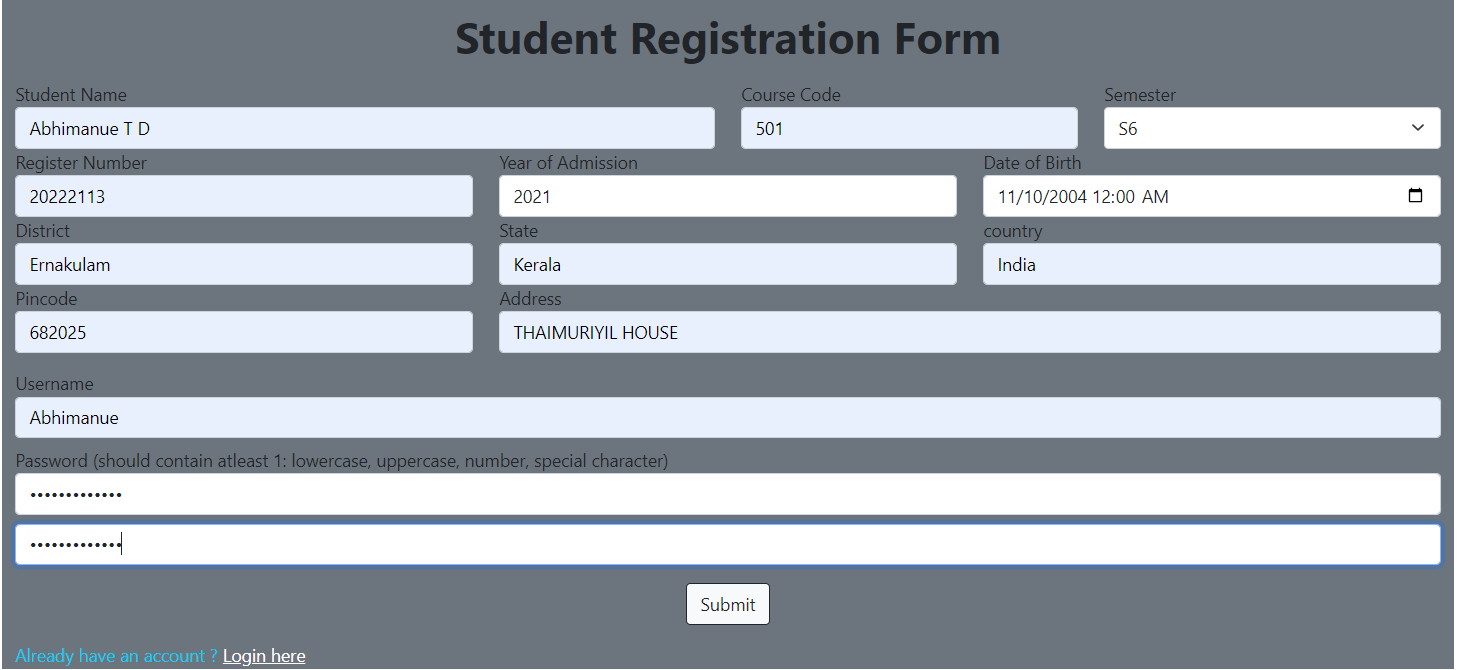
\includegraphics[width=16cm]{Reg.png}
\caption{Student Registration Form}
\label{fig:figure2}
\end{figure}
\begin{verbatim}
    
\end{verbatim}
\newpage
\fancyhead[LO]{\textbf{CYCLE-2, EXPERIMENT-3}}
\fancyhead[RO]{11/06/24}
\begin{flushleft}
\section{CREATE A WEBPAGE FOR STUDENTS REGISTRATION WITH ALL THE FIELDS LR REQUIRED AS PER THE EXPERIMENT IN CYCLE NUMBER 1 FOR STUDENT DATA AND ALSO INCLUDE USERNAME AND PASSWORD IN REGISTRATION FORM AND ALSO HASH THE PASSWORD}
\hrulefill
\vspace{1cm}
\subsection{AIM}
To create a webpage for student registration with all the fields that are required as per the experiment in cycle 1 for student database by creating a form, including user and password fields in the registration form and to encrypt the password with sha512.
\subsection{PROCEDURE}

\subsubsection{Creating tables in database}
\vspace{0.1in}\hspace{0.3in}\$ mysql -u abhimanue\_20222113 -h 192.168.10.222 -p\\
\vspace{0.1in}\hspace{0.4in}\textgreater use abhimanue\_20222113;\\
\vspace{0.2in}
\subsubsection{Table for authentication}
\vspace{0.2in}
\textgreater create table auth(sid int primary key,username varchar(30) unique,password varchar(128),foreign key(sid) references to studentslist(sid));\\
\vspace{0.2in}
\subsubsection{Table for student list}
\vspace{0.2in}
\textgreater create table studentlist(sid int Primary Key,name varchar(30),address text,year year,country varchar(30),course int,district varchar(30),dob date,pincode int,regno int,sem varchar(3),state varchar(30));

\end{flushleft}

\newpage
\fancyhead[LO]{\textbf{CYCLE-2, EXPERIMENT-3}}
\fancyhead[RO]{11/06/24}
\begin{verbatim}
    
\end{verbatim}
\newpage
\begin{flushleft}
\vspace{0.1in}
\subsubsection{HTML file in the nginx root folder}
\vspace{0.1in}
\$ nano /home/20222113/newreg.html \\
In HTML add required headers for bootstrap and link php file using form action reg.php.
Form in POST method inside form required fields for student details and submit button.\\
For Bootstrap.
\begin{verbatim}
    <link rel="stylesheet" href="https://maxcdn.bootstrapcdn.com/
    bootstrap/3.3.7/css/bootstrap.css">
    <style type="text/css">
\end{verbatim}
And password can be hash using  hash('sha512',\$password).\\

\subsubsection{Create php file to use database}
\$ vim /home/20222113/newreg.php\\
Values passed by html will be transfer to database by connecting database.\\
\vspace{0.2in}\begin{verbatim}$con = new mysqli("localhost","20222113","20222113", "abhimanue_20222113"
        , 3306, "") or die ('Could not connect to the database server' . 
            mysqli_connect_error());

    $loginqr = "INSERT INTO studentslist (regno, name, semester, course,
    adm_year,dob, address, district, state, country, pincode) VALUES ("
    . $regno . ", \"" .$name . "\", \"" . $semester . "\", \"" . $course
    . "\", " . $adm_year . ", \"" . $dob . "\", \"" . $address . "\",
    \"" . $district . "\", \"" . $state . "\", \"" . $country . "\", "
    . $pincode . ");";
    
    $statement = $con->prepare($loginqr);
\end{verbatim}
\vspace{1in}
\subsection{RESULT}
Registration form for students with hash function has been successfully implemented.

\end{flushleft}


\newpage
\fancyhead[LO]{\textbf{CYCLE-2, EXPERIMENT-4}}
\fancyhead[RO]{11/06/24}
\begin{flushleft}
\begin{figure}[h]
\vspace{1in}

\includegraphics[width=16cm]{Login.png}
\caption{Student Login}
\label{fig:figure2}
\vspace{1in}
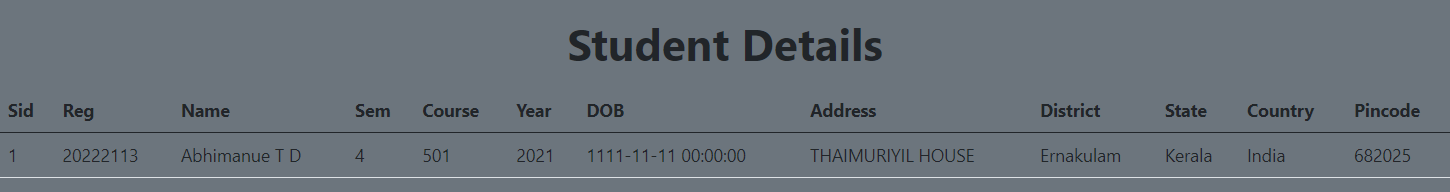
\includegraphics[width=16cm]{Details.png}
\caption{Student Details}
\label{fig:figure2}
\end{figure}
\newpage
\section{CREATE A LOGIN PAGE THAT ACCEPTS THE USERNAME AND PASSWORD FOR STUDENT DATA.IF SUCCESSFULL LOGIN AND SHOW DETAILS}
\hrulefill
\vspace{1cm}
\subsection{AIM}
To create a login page for user and password for student data which displays student details on successfull login.
\subsection{PROCEDURE}
\vspace{0.2in}
\textbullet Create an html file in the nginx root folder which has\\ required field for 'username' and 'password'.\\
\vspace{0.1in}\hspace{0.3in}\$ vim /home/20222113/login.html\\
\hspace{0.2in}\textbullet Creat a php in the nginx root folder\\
\vspace{0.1in}\hspace{0.3in}\$ vim /home/20222113/login.php\\
\hspace{0.2in}\textbullet Check if username and password is correct in table 'auth':\\
\begin{verbatim}
    $doquerry=mysqli_query($con,$query);
    while ($row=mysqli_fetch_array($doquerry)) {
    if(hash('sha512',$password)==$row['password']){
\end{verbatim}\\
\hspace{0.2in}\textbullet Check if details are available in studentslist table:\\
\begin{verbatim}
    while ($row2=mysqli_fetch_array($doquerry2)) {
    if($row['sid']==$row2['sid'])
\end{verbatim}
\hspace{0.2in}\textbullet Then print all values in that row in table.\\
\vspace{1in}
\subsection{RESULT}
Login page for students using php has been successfully implemented.
\end{flushleft}


\end{document}